\chapter{System Architecture}

\begin{figure}
  \centering
  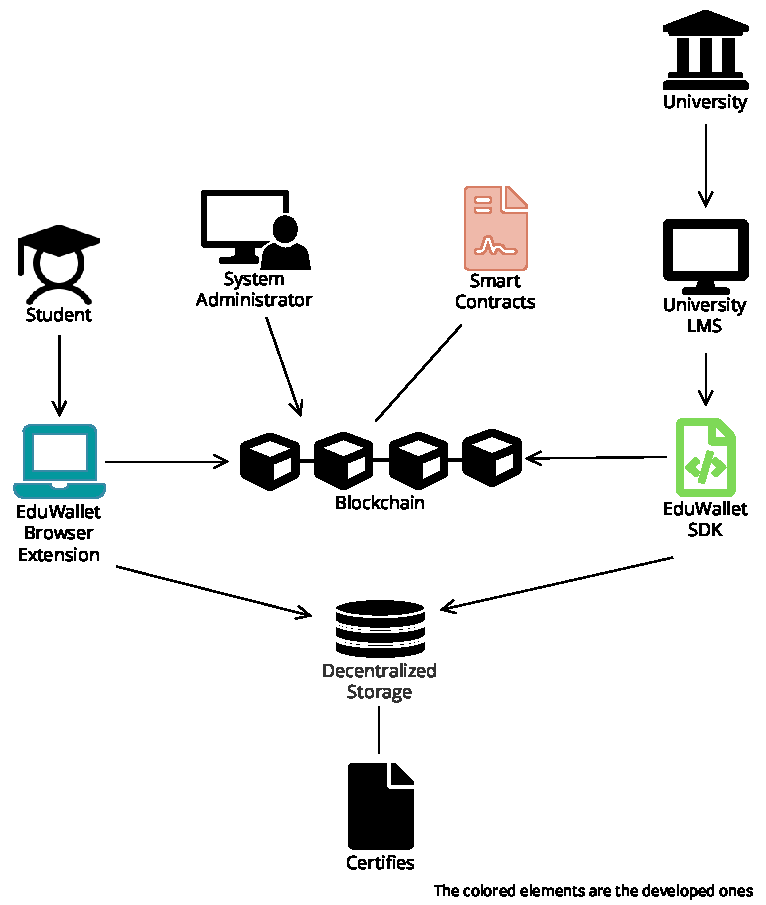
\includegraphics[width=0.6\textwidth]{figures/Architecture diagram basic.pdf}
  \caption[System basic architecture diagram]{Base architecture of the \acrlong{ew} system}
  \label{fig:baseArchDiag}
\end{figure}

This chapter presents an high-level description of the \acrlong{ew} system and its component, developed to address the requirements outlined in \cref{chap:requirements}. The system is composed of several integrated components, as illustrated in \cref{fig:baseArchDiag}:
\begin{itemize}
    \item A set of \textit{smart contracts} responsible for all blockchain-related operations, including \acrshort{sw} creation and transaction management.
    \item A \textit{browser extension} that allows students to manage their academic wallets (see \cref{sec:browserExtensionDesign}).
    \item A \textit{\acrfull{sdk}} designed for universities to interact with the \acrshort{ew} system (see \cref{sec:sdkDesign}).
    \item An external \textit{decentralized storage system} used to store and retrieve certification files (see \cref{sec:decStorageDesgn}).
\end{itemize}

In addition to these core components, we developed a simple yet complete \textit{\acrfull{cli}}, which simulates a university's \acrshort{lms} and its interaction with the academic records system. The \acrshort{cli} serves as a testing and demonstration tool and enables users to perform all operations typically available to universities, thereby simplifying the interaction with our \acrshort{sdk}.

Since the focus of our work is on the interaction of universities and students with the academic registry, the system administrator's core functionalities\footnote{The approval and subscription of universities} have been inserted directly in the \acrshort{cli}. This design decision streamlines our use case and reduces unnecessary complexity.

A more detailed analysis of each component is provided in the following sections.
